\documentclass[11pt,a4paper]{amsart}
\usepackage[utf8]{inputenc}
\usepackage[T1]{fontenc}
\usepackage{mathptmx}
\usepackage[a4paper,margin=2.6cm]{geometry}
\usepackage{microtype}
\usepackage{amsmath,amssymb}
\usepackage{booktabs,array,tabularx,multirow}
\usepackage{enumitem}
\usepackage{graphicx}
\usepackage{tikz}
\usetikzlibrary{arrows.meta,positioning,calc}
\usepackage{pgfplots}
\pgfplotsset{compat=1.17}
\usepackage[hidelinks]{hyperref}

\renewcommand{\abstractname}{Resumen}
\renewcommand{\refname}{Referencias}
\renewcommand{\tablename}{Tabla}
\renewcommand{\figurename}{Figura}
\renewcommand{\contentsname}{Contenido}
\renewcommand{\appendixname}{Apéndice}

\setlength{\parindent}{1.2em}
\setlist{itemsep=1pt,topsep=3pt,leftmargin=1.8em}
\renewcommand{\arraystretch}{1.12}
\emergencystretch=2em

\newcommand{\gr}{$^{\circ}$}
\newcommand{\Mae}{\mathrm{MAE}}
\newcommand{\R}{\mathbb{R}}

\makeatletter\def\@@and{y}\makeatother
\begin{document}

\title[Autoencoder recurrente de ciclos de marcha]{Autoencoder recurrente para ciclos de marcha: diagn\'ostico, cierre del ciclo y evaluaci\'on de un codificador fundacional congelado}

\author{Jes\'us David Cantell\'on Espitia}
\thanks{Universidad EAFIT, Pr\'actica Investigativa III. Noviembre de 2026.}
\author{Juan David Mart\'inez Vargas}

\begin{abstract}
Se estudia un autoencoder recurrente (GRU) que modela ciclos completos de marcha de seis ángulos articulares remuestreados a 101 puntos, con el fin de obtener un modelo normativo del grupo control. En la comparación inicial del proyecto, las dos variantes recurrentes (con ciclos limpios y con eliminación de ruido) tuvieron los mayores errores de reconstrucción entre los modelos que aprenden de los datos, y reconstruían ciclos cuyos extremos no coinciden. Se identificaron dos causas probables, a saber, que el código latente solo entra al decodificador como estado inicial y que la pérdida no exige periodicidad, y se propusieron dos modificaciones: entregar el código en cada paso del decodificador y añadir a la pérdida un término de cierre del ciclo. Con cinco semillas y prueba t pareada, el error absoluto medio del modelo limpio bajó de 4.99\gr{} (modelo original reproducido) a 4.11\gr{} (3.91\gr{} con un ensamble de cinco modelos) y el salto entre el primer y el último punto de 5.07\gr{} a 0.87\gr{}. En la variante con eliminación de ruido, el salto bajó de 3.04\gr{} a 0.57\gr{} y la ganancia de corrección de 0.296 a 0.337. Un conjunto amplio de componentes adicionales no aportó mejoras, lo que sugiere que el límite actual es el tamaño de los datos (240 ciclos de entrenamiento). Un modelo fundacional de series de tiempo (TimesFM 2.5) usado como codificador congelado no mejoró los resultados: su error fue igual al de pesos aleatorios y mayor que el del GRU. Un control no planeado, una proyección lineal de la serie cruda con el mismo decodificador, obtuvo un error menor que el del codificador recurrente, lo que indica que este no es el factor que limita el rendimiento. Se discuten las limitaciones del diseño, entre ellas la selección de hiperparámetros sobre el conjunto de prueba de control.
\end{abstract}

\maketitle

\noindent\textbf{Palabras clave:} análisis de marcha, autoencoder, red recurrente, modelo normativo, cierre de ciclo, modelo fundacional de series de tiempo.

\medskip
\noindent\textbf{Abstract.}\ \textit{A recurrent (GRU) autoencoder for gait cycles of six joint angles resampled to 101 points is studied as a normative model of the control group. In the project's initial comparison, the two recurrent variants showed the largest reconstruction errors among the learned models and produced cycles whose endpoints did not match. Two probable causes were identified and two modifications proposed: feeding the latent code to the decoder at every step and adding a cycle-closure term to the loss. With five seeds and paired t-tests, the clean model's mean absolute error decreased to 4.11\gr{} (3.91\gr{} with a five-model ensemble) and the endpoint jump to 0.87\gr{}; in the denoising variant the jump decreased to 0.57\gr{} and the correction gain increased to 0.337. Many additional components brought no improvement, suggesting that data size is the current limit. A frozen time-series foundation model (TimesFM 2.5) used as encoder did not improve results: its error matched that of random weights and exceeded that of the GRU. An unplanned control, a linear projection of the raw series with the same decoder, achieved a lower reconstruction error than the recurrent encoder. Limitations, including hyperparameter selection on the control test set, are discussed.}

%--------------------------------------------------------------------
\section{Introducción}

El análisis de la marcha con apoyo de aprendizaje profundo es una línea activa para el control de exoesqueletos pediátricos y la caracterización de patologías motoras. Una estrategia es aprender la marcha de referencia a partir de personas sin patología y usarla como trayectoria objetivo del dispositivo \cite{kolaghassi2023}. En el proyecto NeuroStrideAI, en cuyo marco se realiza este trabajo, se desarrollaron además un clasificador de las formas de diplejía espástica \cite{ferrari2019} y un pipeline de estimación de ángulos articulares a partir de video.

En este trabajo cada ciclo de marcha se trata como un punto de $\R^{101\times 6}$ (101 instantes del ciclo y seis ángulos articulares) y se estudia un modelo de variedad de ciclos: un autoencoder que comprime el ciclo en un código latente de pocos números y lo reconstruye \cite{hinton2006}. La comparación inicial del proyecto \cite{neurostride2026} evaluó siete modelos sobre los mismos datos. Entre los que aprenden de los datos, las dos variantes del autoencoder recurrente (modelo A, entrenado con ciclos limpios, y modelo B, entrenado con ciclos dañados para corregirlos \cite{vincent2008}) tuvieron los mayores errores de reconstrucción (error absoluto medio de 5.17\gr{} y 5.35\gr{}) y saltos de 4.94\gr{} y 3.45\gr{} entre el primer y el último punto del ciclo reconstruido, aunque un ciclo de marcha es una curva periódica.

\textbf{Trabajo previo y contribución.} Este estudio se apoya en el trabajo previo del equipo del proyecto: el pipeline de procesamiento (estimación de pose, ángulos articulares y segmentación de ciclos), la preparación del conjunto de ciclos con su control de calidad y partición por sujeto, y la comparación inicial de siete modelos con tres evaluaciones \cite{neurostride2026}. Las contribuciones de este informe son:
\begin{enumerate}[label=(\roman*)]
\item el diagnóstico de dos limitaciones del autoencoder recurrente y dos modificaciones que las corrigen (sección~\ref{sec:mods});
\item un protocolo de validación con cinco semillas y prueba t pareada, y métricas adicionales de forma del ciclo;
\item un estudio negativo de componentes adicionales que delimita dónde está el cuello de botella (sección~\ref{sec:negativos});
\item la evaluación de un modelo fundacional de series de tiempo como codificador congelado, junto con dos controles (sección~\ref{sec:fundacional}).
\end{enumerate}

El documento se organiza así: la sección~\ref{sec:relacionado} resume el trabajo relacionado; la~\ref{sec:datos} describe los datos; la~\ref{sec:metodos} los modelos; la~\ref{sec:protocolo} el protocolo y las métricas; la~\ref{sec:resultados} los resultados; y las secciones~\ref{sec:discusion} a~\ref{sec:conclusiones} la discusión, las limitaciones y las conclusiones.

%--------------------------------------------------------------------
\section{Trabajo relacionado}
\label{sec:relacionado}

\textbf{Autoencoders.} Un autoencoder aprende una representación comprimida minimizando el error de reconstrucción \cite{hinton2006}; la variante con eliminación de ruido recibe una entrada dañada y reconstruye la versión limpia \cite{vincent2008}. Para secuencias se usan codificadores y decodificadores recurrentes, en particular unidades recurrentes con compuertas (GRU) \cite{cho2014}, a veces bidireccionales \cite{schuster1997}.

\textbf{Marcha de referencia.} Kolaghassi et al. \cite{kolaghassi2023} aprenden trayectorias de marcha estables como referencia para exoesqueletos pediátricos con parálisis cerebral, y Ferrari et al. \cite{ferrari2019} clasifican la diplejía espástica con redes recurrentes. Estos trabajos motivan un modelo normativo de ciclos completos, que es el objeto de este informe.

\textbf{Modelos fundacionales de series de tiempo.} Modelos preentrenados con grandes colecciones de series, como TimesFM \cite{das2024timesfm}, MOMENT \cite{goswami2024moment} y Chronos \cite{ansari2024chronos}, se proponen para pronóstico y, en el caso de MOMENT, también para extraer representaciones y reconstruir. En este informe solo se evalúa TimesFM, que es el modelo sugerido para el proyecto; la conclusión se limita a ese modelo y a un diseño de uso concreto (sección~\ref{sec:fundacional}).

%--------------------------------------------------------------------
\section{Datos}
\label{sec:datos}

\subsection{Construcción de los ciclos}

Los datos proceden del pipeline del proyecto: video de marcha, estimación de pose con AlphaPose \cite{fang2023alphapose} y ángulos articulares en el plano sagital muestreados a 30 Hz. Se usan seis señales: flexo-extensión de cadera y rodilla, y dorsiflexión-plantarflexión de tobillo, para las piernas izquierda y derecha. Cada intervalo de ciclo de la segmentación original se trata como un ciclo independiente y se interpola a 101 puntos (0 a 100\% del ciclo) con el interpolador PCHIP \cite{fritsch1980}, que conserva picos y monotonía.

Un ciclo se acepta si cumple un control de calidad: entre 15 y 90 cuadros crudos, al menos 90\% de valores finitos y, en cada una de las seis señales, un salto absoluto máximo entre cuadros consecutivos de 17\gr{} y una diferencia entre el primer y el último valor no mayor de 25\gr{}. Los umbrales se derivaron de auditar los 551 intervalos originales. Quedan 461 ciclos válidos de 64 personas. La etiqueta del sujeto (control o caso) se deriva del identificador de origen del reporte de migración del proyecto; no se leen nombres ni otros identificadores personales.

\subsection{Partición por sujeto}

La partición se hace por sujeto para evitar que ciclos de una misma persona aparezcan en conjuntos distintos \cite{saeb2017}. Los sujetos control se dividen aleatoriamente (semilla 42) en 70\% para entrenamiento, 15\% para validación y 15\% para prueba. Los sujetos del grupo de casos (niños con parálisis cerebral) se reservan como conjunto de prueba externo y nunca intervienen en el ajuste.

\begin{table}[h]
\centering\small
\begin{tabular}{llcc}
\toprule
Conjunto & Grupo & Sujetos & Ciclos \\
\midrule
Entrenamiento & control & 28 & 240 \\
Validación & control & 6 & 44 \\
Prueba de control & control & 7 & 47 \\
Prueba externa & casos & 23 & 130 \\
\midrule
Total & & 64 & 461 \\
\bottomrule
\end{tabular}
\caption{Partición por sujeto.}
\label{tab:particion}
\end{table}

\subsection{Estandarización}

Cada una de las seis señales se estandariza con la media y la desviación estándar de los ciclos de entrenamiento (todas las fases), con un mínimo de $10^{-4}$ para la desviación. Los modelos se entrenan y operan en unidades estandarizadas; las métricas en grados se calculan tras invertir la estandarización.

%--------------------------------------------------------------------
\section{Métodos}
\label{sec:metodos}

Sea $G\in\R^{101\times 6}$ un ciclo estandarizado, $g_t\in\R^6$ su fila $t$ y $\tau_t=(t-1)/100$ la fase.

\subsection{Modelos de referencia}

Los modelos de referencia son los de la comparación inicial del proyecto \cite{neurostride2026}, entrenados solo con ciclos de control de entrenamiento.
\begin{itemize}
\item \textit{Media de controles:} el ciclo promedio por fase.
\item \textit{PCA} \cite{jolliffe2016}: proyección lineal del ciclo aplanado (606 valores) con el menor número de componentes que explique 95\% de la varianza, con un máximo de 20.
\item \textit{Autoencoder convolucional} unidimensional con código de 16 valores \cite{hinton2006} y su variante \textit{denoising} \cite{vincent2008}.
\item \textit{Proceso gaussiano periódico} \cite{rasmussen2006}: media de controles más un residuo modelado con el núcleo $k(t,t')=\sigma_f^2\exp\!\big(-2\sin^2(\pi|t-t'|)/\ell^2\big)+\sigma_n^2\delta(t,t')$. El largo de escala $\ell$ proviene de un ajuste previo del proyecto por máxima verosimilitud, $\sigma_f^2$ es la varianza empírica del residuo, y $\sigma_n^2=\lambda\sigma_f^2$ se selecciona en validación maximizando la ganancia de corrección.
\end{itemize}

\subsection{Autoencoder recurrente base (modelo A)}

El codificador es una GRU bidireccional de una capa con 48 unidades ocultas por dirección, que lee el ciclo de $t=1$ a $101$ con las seis señales como entrada. Los estados finales de ambas direcciones se concatenan y una capa lineal produce el código $z\in\R^{d}$ ($d=16$ en el modelo base):
\begin{equation}
z = W_e\,[\overrightarrow{h}_{101};\overleftarrow{h}_{1}] + b_e .
\end{equation}
El decodificador es una GRU de 48 unidades. Su estado inicial se obtiene del código, $h_0=W_0 z+b_0$, y en cada paso recibe una codificación periódica de la fase, $u_t=[\sin 2\pi\tau_t,\ \cos 2\pi\tau_t]$:
\begin{equation}
h_t=\mathrm{GRU}(h_{t-1},u_t),\qquad \hat g_t = W_o h_t + b_o .
\end{equation}
La pérdida base es el error cuadrático medio entre $\hat G$ y $G$ en unidades estandarizadas; el error absoluto medio en grados es solo una métrica de evaluación. El modelo A se entrena con ciclos limpios (entrada y objetivo iguales).

\subsection{Variante con eliminación de ruido (modelo B)}
\label{sec:denoising}

El modelo B tiene la misma arquitectura, pero recibe como entrada un ciclo dañado $\tilde G$ y su objetivo es el ciclo limpio $G$. En cada lote, y para cada canal $c$, el daño es
\begin{equation}
\tilde g_{t,c}=m_c+a_c\,(g_{t,c}-m_c)+b_c+\varepsilon_{t,c},
\end{equation}
donde $m_c$ es la media del canal en el ciclo, $a_c\sim U(0.5,1.8)$ es un cambio de amplitud, $b_c\sim U(-0.9,0.9)$ un desplazamiento vertical y $\varepsilon_{t,c}\sim\mathcal N(0,0.15^2)$ ruido. Después, los tres canales de cada pierna se desplazan circularmente un número entero de pasos $s\sim U\{-8,\dots,8\}$, de forma independiente por pierna. La validación y la parada temprana usan ciclos limpios como entrada.

\subsection{Modificaciones propuestas}
\label{sec:mods}

\textbf{Modificación 1: código en cada paso del decodificador.} Se concatena $z$ a la entrada del decodificador en los 101 pasos, $u_t'=[\sin 2\pi\tau_t,\ \cos 2\pi\tau_t,\ z]$, conservando $h_0=W_0z+b_0$ y la codificación de fase. La motivación es que, con $z$ solo en el estado inicial, la información del código debe sobrevivir a 100 actualizaciones recurrentes. Un intento previo del proyecto \cite{neurostride2026}, que alimentaba el decodificador únicamente con $z$ repetido y sin señal de fase, no funcionó; la modificación propuesta mantiene la codificación de fase y el estado inicial derivado del código.

\textbf{Modificación 2: pérdida de cierre.} Un ciclo de marcha es periódico: el punto 101 y el punto 1 son vecinos en el tiempo. Se añade a la pérdida un término de cierre con peso $w\ge 0$:
\begin{equation}
\mathcal L=\frac{1}{606}\sum_{t=1}^{101}\sum_{c=1}^{6}(\hat g_{t,c}-g_{t,c})^2+w\cdot\frac16\sum_{c=1}^{6}\left|\hat g_{1,c}-\hat g_{101,c}\right| ,
\end{equation}
promediada sobre el lote. El peso $w$ regula el compromiso entre fidelidad y cierre. Las configuraciones finales son $d=32$ y $w=0.1$ para el modelo A, y $d=16$ y $w=0.05$ para el modelo B.

\textbf{Ensamble.} Un ensamble promedia las predicciones de cinco modelos entrenados con semillas distintas \cite{dietterich2000}.

\begin{figure}[t]
\centering
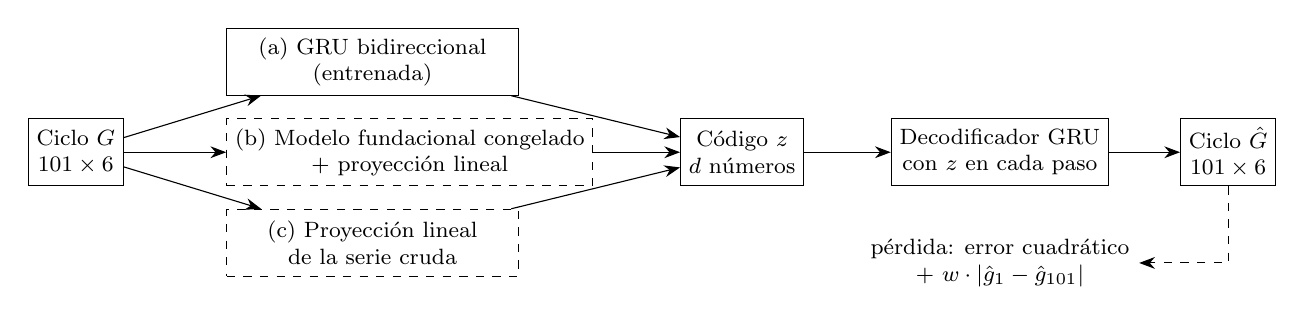
\begin{tikzpicture}[
 box/.style={draw,rectangle,minimum height=0.85cm,align=center,font=\footnotesize,inner sep=3pt},
 arr/.style={-{Stealth[length=2mm]}}]
\node[box] (in) {Ciclo $G$\\ $101\times 6$};
\node[box,right=1.3cm of in,yshift=1.15cm,minimum width=3.7cm] (e1) {(a) GRU bidireccional\\ (entrenada)};
\node[box,right=1.3cm of in,minimum width=3.7cm,dashed] (e2) {(b) Modelo fundacional congelado\\ + proyección lineal};
\node[box,right=1.3cm of in,yshift=-1.15cm,minimum width=3.7cm,dashed] (e3) {(c) Proyección lineal\\ de la serie cruda};
\node[box,right=1.1cm of e2] (z) {Código $z$\\ $d$ números};
\node[box,right=1.1cm of z,minimum width=2.5cm] (dec) {Decodificador GRU\\ con $z$ en cada paso};
\node[box,right=0.9cm of dec] (out) {Ciclo $\hat G$\\ $101\times 6$};
\draw[arr] (in) -- (e1); \draw[arr] (in) -- (e2); \draw[arr] (in) -- (e3);
\draw[arr] (e1) -- (z); \draw[arr] (e2) -- (z); \draw[arr] (e3) -- (z);
\draw[arr] (z) -- (dec); \draw[arr] (dec) -- (out);
\node[font=\footnotesize,align=center,below=0.55cm of dec] (loss) {pérdida: error cuadrático\\ $+\ w\cdot|\hat g_1-\hat g_{101}|$};
\draw[arr,dashed] (out.south) |- (loss.east);
\end{tikzpicture}
\caption{Esquema del autoencoder. Se compara un mismo decodificador con tres codificadores: (a) la GRU recurrente de los modelos A y B, (b) un modelo fundacional congelado con proyección lineal entrenable y (c) una proyección lineal de la serie cruda (control). Las líneas discontinuas indican las alternativas evaluadas en la sección~\ref{sec:fundacional}.}
\label{fig:esquema}
\end{figure}

\subsection{Componentes adicionales explorados}

Para delimitar dónde está el cuello de botella se probaron componentes adicionales con el mismo protocolo, de forma exploratoria (una semilla) y, si resultaron prometedores, con cinco semillas.
\begin{itemize}
\item \textit{Regularizaciones de diferencias consecutivas} ($t$ frente a $t-1$), con las diferencias circulares $\Delta g_t=g_{t+1}-g_t$ (índices módulo 101): suavidad circular $\lambda\,\overline{|\Delta\hat g|}$; curvatura circular $\lambda\,\overline{|\Delta^2\hat g|}$; igualar incrementos $\lambda\,\overline{|\Delta\hat g-\Delta g|}$; igualar la pendiente en la costura, $\lambda\,\overline{|(\hat g_2-\hat g_1)-(\hat g_{101}-\hat g_{100})|}$; un término de núcleo periódico $\lambda\sum_{s,t}K(\tau_s,\tau_t)\|\hat g_s-\hat g_t\|^2$ con $K\propto\exp(-2\sin^2(\pi(\tau_s-\tau_t))/\ell^2)$ y $\ell=0.15$; y una ponderación del error cerca de los extremos del ciclo.
\item \textit{Cambios de arquitectura y entradas:} decodificador bidireccional, atención en el codificador \cite{bahdanau2015}, y velocidad angular y asimetría izquierda-derecha como entradas adicionales.
\item \textit{Cambios de entrenamiento del modelo B:} penalización de consistencia entre los códigos del ciclo limpio y del dañado, intensidad del daño (0.5, 1.0 y 1.5) y currículo de daño creciente.
\end{itemize}

\subsection{Codificador fundacional congelado}
\label{sec:fundacional_met}

Se evaluó TimesFM 2.5 \cite{das2024timesfm} (200 millones de parámetros, 20 bloques de transformador con atención causal, parches de 32 puntos, pesos con licencia Apache 2.0) como codificador congelado. El diseño es el siguiente.
\begin{enumerate}
\item Cada una de las seis señales estandarizadas se trata como una serie univariada de 101 puntos, que se remuestrea linealmente a 128 puntos (cuatro parches de 32). El modelo normaliza internamente cada serie por instancia, por lo que descarta su nivel y su escala; para conservarlos se añaden la media y la desviación estándar de la serie.
\item Se toma el estado oculto de un bloque del modelo, se promedian los cuatro parches y se añade el estado del último parche (1280 valores cada uno). Con los dos estadísticos, cada canal aporta 2562 características, y los seis canales suman 15\,372.
\item Una capa lineal entrenable proyecta esas características estandarizadas al código $z$ ($d=32$ en el tipo A y $d=16$ en el tipo B).
\item Se usa el decodificador del modelo mejorado (modificaciones 1 y 2), entrenado desde cero, con la misma pérdida y el mismo protocolo. En el tipo B, las características se recalculan en cada lote sobre el ciclo dañado.
\end{enumerate}
El bloque (último o décimo), la forma de agrupar los parches (promedio, o promedio y último) y el decaimiento de pesos ($0$ o $10^{-3}$) se eligieron entre ocho configuraciones con el conjunto de validación y una semilla, sin usar el conjunto de prueba. La verificación de que los pesos se cargaron correctamente consistió en pronosticar 32 puntos de una onda seno: el error medio absoluto fue 0.036 con los pesos preentrenados y 1.877 con pesos aleatorios.

\subsection{Controles}

Para interpretar el resultado se añadieron dos controles con el mismo decodificador, la misma pérdida y las mismas semillas: (i) \textit{TimesFM con pesos aleatorios} (misma arquitectura y extracción de características, sin preentrenamiento, con las escalas de las normas internas fijadas en uno), que separa el aporte del preentrenamiento del de la arquitectura; y (ii) \textit{serie cruda}, en la que la serie estandarizada y aplanada (606 valores) entra directamente a la proyección lineal, lo que indica qué se logra sin ningún modelo preentrenado. Una primera versión del control de pesos aleatorios usó la inicialización por defecto de la biblioteca, en la que las escalas de las normas internas valen cero y los bloques del transformador actúan como identidad; se corrigió y el control se repitió con las cinco semillas. Las conclusiones no cambiaron: el error del control inicial fue 7.14\gr{} y el del corregido, 7.23\gr.

%--------------------------------------------------------------------
\section{Protocolo experimental y métricas}
\label{sec:protocolo}

\subsection{Entrenamiento, semillas y contraste estadístico}

Las redes se implementan en PyTorch \cite{paszke2019} y se entrenan con Adam \cite{kingma2015}, tasa de aprendizaje $10^{-3}$, lotes de 64 ciclos, hasta 100 épocas, recorte de la norma del gradiente a 1.0 \cite{pascanu2013} y parada temprana con paciencia de 12 épocas sobre la pérdida de validación \cite{prechelt1998}; se conservan los pesos de la mejor época. PCA y el proceso gaussiano se ajustan con scikit-learn \cite{pedregosa2011}.

La inicialización y el orden de los lotes dependen de una semilla. Para afirmar una mejora se entrena cada configuración con cinco semillas (42, 1, 7, 123 y 2024) y se compara con la referencia semilla a semilla mediante una prueba t pareada de dos colas \cite{student1908} con $\alpha=0.05$. La exploración inicial de variantes usa una sola semilla (42) y sus resultados no se consideran evidencia. No se corrige por comparaciones múltiples.

\subsection{Métricas}

Todas las métricas son las mismas para todos los modelos. Las métricas en grados se calculan tras invertir la estandarización; $N$ es el número de ciclos del conjunto evaluado.

\textit{Evaluación I: fidelidad} (47 ciclos limpios de prueba de control):
\begin{align}
\Mae&=\frac{1}{606N}\sum_{n}\sum_{t,c}\left|\hat g^{(n)}_{t,c}-g^{(n)}_{t,c}\right|,\\
\text{Salto de cierre}&=\frac{1}{6N}\sum_{n}\sum_{c}\left|\hat g^{(n)}_{1,c}-\hat g^{(n)}_{101,c}\right|.
\end{align}
Se reporta también la raíz del error cuadrático medio (RMSE).

\textit{Evaluación II: corrección} (los mismos 47 ciclos, dañados con la receta de la sección~\ref{sec:denoising}, con una realización aleatoria fija):
\begin{equation}
\text{Ganancia de corrección}=1-\frac{\Mae(f(\tilde G),G)}{\Mae(\tilde G,G)} ,
\end{equation}
donde $f$ es el modelo; 0 significa que no se deshace nada del daño y 1 que se deshace por completo.

\textit{Evaluación III: casos externos} (130 ciclos del grupo de casos). Sea $d(x)$ la distancia euclídea, en unidades estandarizadas y con el ciclo aplanado, entre $x$ y el ciclo de control de entrenamiento más cercano:
\begin{align}
\text{Ganancia de tipicidad}&=\frac1N\sum_{n}\left(1-\frac{d(f(x^{(n)}))}{d(x^{(n)})}\right),\\
\text{Intervención}&=\frac{1}{606N}\sum_{n}\sum_{t,c}\left|f(x^{(n)})_{t,c}-x^{(n)}_{t,c}\right|\ \text{(en grados)}.
\end{align}
La intervención describe cuánto cambia el modelo la entrada y no tiene sentido de ``mejor''.

\textit{Métricas de forma} (en grados, menor es mejor): \emph{pendiente en la costura}, $|(\hat g_2-\hat g_1)-(\hat g_{101}-\hat g_{100})|$ promediada; \emph{error en incrementos}, $\overline{|\Delta\hat g-\Delta g|}$ sin cierre circular; y \emph{rugosidad}, $\overline{|\Delta^2\hat g|}$.

\subsection{Hipótesis}

\begin{enumerate}[label=\textbf{H\arabic*.},leftmargin=2.2em]
\item Entregar el código $z$ en cada paso del decodificador reduce el error de reconstrucción en ciclos de control no vistos.
\item El término de cierre reduce el salto de cierre, y existe un peso $w$ para el cual el error de reconstrucción no empeora de forma apreciable.
\item Las dos modificaciones aplicadas a la variante con eliminación de ruido reducen el salto de cierre y aumentan la ganancia de corrección.
\item Un ensamble de cinco modelos reduce el error y el salto frente a un modelo individual.
\item Un codificador fundacional congelado, con un decodificador entrenado sobre sus representaciones, mejora al menos una métrica de fidelidad o de corrección frente al autoencoder recurrente mejorado.
\end{enumerate}

%--------------------------------------------------------------------
\section{Resultados}
\label{sec:resultados}

\subsection{Punto de partida}

La tabla~\ref{tab:inicial} reproduce la comparación inicial del proyecto \cite{neurostride2026}, con una sola corrida por modelo. Entre los modelos que aprenden de los datos, A y B tienen el mayor error (5.17\gr{} y 5.35\gr{}) y saltos de cierre de 4.94\gr{} y 3.45\gr{}, frente a 3.41\gr{} de PCA. La media de controles no aprende nada; su salto bajo (0.60\gr{}) es trivial, porque su salida es un promedio de ciclos. El mejor error corresponde a PCA (2.78\gr{}) y la mayor ganancia de corrección al autoencoder convolucional con eliminación de ruido (0.412).

\begin{table}[h]
\centering\small
\setlength{\tabcolsep}{4pt}
\begin{tabular}{lccccc}
\toprule
 & MAE (\gr) & Salto (\gr) & Corrección & Tipicidad & Intervención (\gr) \\
\midrule
Media de controles & 8.77 & \textbf{0.60} & $-0.121$ & 0.132 & 10.83 \\
PCA & \textbf{2.78} & 3.41 & 0.207 & 0.127 & 3.86 \\
Autoencoder convolucional & 3.30 & 3.11 & 0.252 & 0.182 & 4.83 \\
Autoencoder convolucional denoising & 4.07 & 1.88 & \textbf{0.412} & 0.376 & 5.98 \\
Proceso gaussiano periódico & 3.30 & \textbf{0.60} & 0.215 & 0.192 & 3.86 \\
Modelo A (GRU) & 5.17 & 4.94 & 0.152 & 0.349 & 8.12 \\
Modelo B (GRU denoising) & 5.35 & 3.45 & 0.280 & 0.385 & 7.89 \\
\bottomrule
\end{tabular}
\caption{Comparación inicial de siete modelos (una corrida por modelo). En negrilla, el mejor valor de cada columna. La intervención no tiene un valor ``mejor''.}
\label{tab:inicial}
\end{table}

Al reproducir los modelos A y B con el protocolo de cinco semillas, con datos reconstruidos a partir de los archivos entregados, las cifras difieren ligeramente de las iniciales (tabla~\ref{tab:origrep}). La comparación de las secciones siguientes usa esta reproducción como referencia, porque aplica exactamente el mismo protocolo que los modelos modificados.

\begin{table}[h]
\centering\small
\setlength{\tabcolsep}{3pt}
\begin{tabular}{llccccc}
\toprule
 & & MAE (\gr) & Salto (\gr) & Corrección & Tipicidad & Interv. (\gr) \\
\midrule
\multirow{3}{*}{Modelo A} & Original reproducido & $4.99\pm0.23$ & $5.07\pm0.55$ & $0.208\pm0.018$ & $0.345\pm0.008$ & $7.78\pm0.13$ \\
 & Mejorado & $4.11\pm0.05$ & $0.87\pm0.11$ & $0.189\pm0.012$ & $0.326\pm0.007$ & $6.14\pm0.10$ \\
 & Valor $p$ & 0.001 & $<0.001$ & 0.077 & 0.034 & $<0.001$ \\
\midrule
\multirow{3}{*}{Modelo B} & Original reproducido & $5.25\pm0.10$ & $3.04\pm0.31$ & $0.296\pm0.014$ & $0.383\pm0.004$ & $7.87\pm0.12$ \\
 & Mejorado & $4.83\pm0.07$ & $0.57\pm0.05$ & $0.337\pm0.007$ & $0.414\pm0.008$ & $7.09\pm0.10$ \\
 & Valor $p$ & $<0.001$ & $<0.001$ & 0.002 & 0.001 & $<0.001$ \\
\bottomrule
\end{tabular}
\caption{Modelos originales reproducidos frente a los mejorados (modelo A: $d=32$, $w=0.1$; modelo B: $d=16$, $w=0.05$), con el mismo protocolo, las mismas semillas y las mismas métricas. Media $\pm$ desviación estándar de cinco semillas; el valor $p$ es de la prueba t pareada.}
\label{tab:origrep}
\end{table}

Una repetición anterior de los modelos originales dio errores de $5.01\pm0.22$\gr{} (A) y $5.20\pm0.07$\gr{} (B), dentro de la variabilidad entre corridas.

\subsection{Mejoras del decodificador: código en cada paso y cierre}
\label{sec:res_mejoras}

\textbf{Modificación 1.} Con una semilla, entregar $z$ en cada paso redujo el error de 4.84\gr{} a 4.22\gr{} y el salto de 4.75\gr{} a 3.91\gr{} (el modelo original varía en $\pm0.56$\gr{} entre semillas). Esta modificación mejora sobre todo la fidelidad, pero no obliga a cerrar el ciclo.

\textbf{Modificación 2.} La figura~\ref{fig:w} muestra el compromiso al variar $w$ (una semilla, solo con la pérdida de cierre). Con $w$ pequeño (0.05 a 0.1) el salto cae de 4.75\gr{} a entre 2.3\gr{} y 1.0\gr{}, y el error cambia poco; con $w\ge0.3$ el error crece de forma clara. El valor $w=0.05$ dio 4.67\gr{} y $w=0.1$ dio 5.23\gr{}, pero con una sola semilla esas diferencias están dentro del ruido.

\begin{figure}[h]
\centering
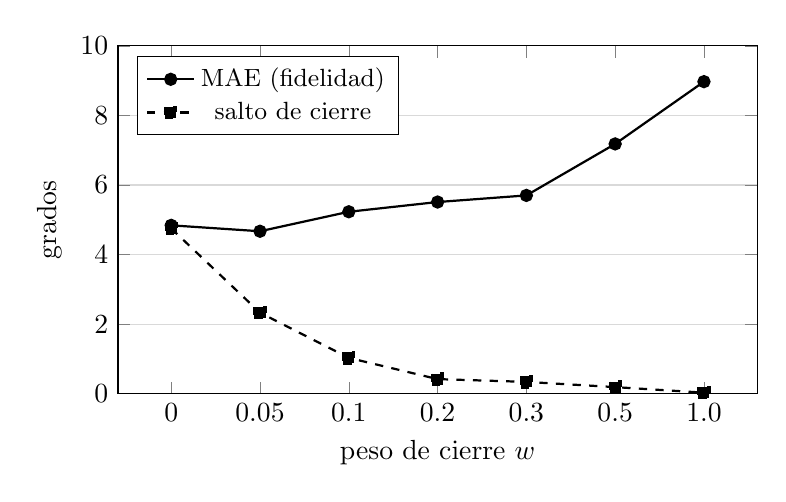
\begin{tikzpicture}
\begin{axis}[width=0.8\textwidth,height=6cm,xlabel={peso de cierre $w$},ylabel={grados},
 symbolic x coords={0,0.05,0.1,0.2,0.3,0.5,1.0},xtick=data,ymin=0,ymax=10,legend pos=north west,
 ymajorgrids,grid style={gray!30},legend style={font=\small}]
\addplot[color=black,mark=*,thick] coordinates {(0,4.84)(0.05,4.67)(0.1,5.23)(0.2,5.51)(0.3,5.70)(0.5,7.18)(1.0,8.97)};
\addlegendentry{MAE (fidelidad)}
\addplot[color=black,mark=square*,thick,dashed] coordinates {(0,4.75)(0.05,2.33)(0.1,1.03)(0.2,0.42)(0.3,0.34)(0.5,0.19)(1.0,0.03)};
\addlegendentry{salto de cierre}
\end{axis}
\end{tikzpicture}
\caption{Compromiso entre fidelidad y cierre al variar el peso $w$ (una semilla).}
\label{fig:w}
\end{figure}

\textbf{Combinación (H1 y H2).} Con las dos modificaciones y $d=16$, $w=0.05$, el error es $4.20\pm0.03$\gr{} y el salto $1.33\pm0.15$\gr{}, frente a $4.99\pm0.23$\gr{} y $5.07\pm0.55$\gr{} del modelo original reproducido; la combinación gana en las cinco semillas en ambas métricas y la dispersión entre semillas del error cae de $\pm0.23$\gr{} a $\pm0.03$\gr{}. Al pasar a $d=32$ y re-ajustar $w=0.1$, el error baja a $4.11\pm0.05$\gr{} ($p=0.018$ frente a $d=16$) y el salto a $0.87\pm0.11$\gr{} ($p=0.004$). Frente al modelo original reproducido, el modelo A mejorado reduce el error en $17.6\%$ y el salto en $82.9\%$ (tabla~\ref{tab:origrep}). El mejor $w$ depende del tamaño del código: con 32 números la red tiene más libertad para ignorar el cierre, por lo que el término debe ser más exigente. H1 y H2 se confirman en la combinación; por separado solo se exploraron con una semilla.

\textbf{Corrección y tipicidad del modelo A.} La mejora de A es de fidelidad y de cierre. Su ganancia de corrección no mejora de forma significativa ($0.208\to0.189$; $p=0.077$) y su ganancia de tipicidad es algo menor ($0.345\to0.326$; $p=0.034$, sin corrección por multiplicidad, en cinco de cinco semillas), mientras que la intervención baja de 7.78\gr{} a 6.14\gr. Es decir, el modelo mejorado copia con más fidelidad y se aleja menos de la entrada; no se probó una explicación de por qué esto reduce la tipicidad.

\subsection{Variante con eliminación de ruido (H3)}

Las mismas modificaciones aplicadas al modelo B ($d=16$, $w=0.05$) mejoran en las cinco semillas el error ($5.25\to4.83$\gr), el salto ($3.04\to0.57$\gr), la ganancia de corrección ($0.296\to0.337$) y la de tipicidad ($0.383\to0.414$), todos con $p\le0.002$ (tabla~\ref{tab:origrep} y apéndice~\ref{app:semillas}); frente a la reproducción original, el error baja $8.0\%$ y el salto $81.4\%$. Un peso $w=0.07$ baja el salto de $0.57\pm0.05$\gr{} a $0.47\pm0.09$\gr{} ($p=0.022$, cuatro de cinco semillas) sin cambio apreciable en el error ($p=0.57$). La mejora en corrección es modesta en términos absolutos; su techo parece estar determinado por qué tan bien el modelo estima el ciclo limpio a partir de uno dañado. H3 se confirma.

\subsection{Ensambles (H4)}

Promediar las predicciones de cinco modelos reduce el error del modelo A a 3.91\gr{} (salto 0.55\gr{}) y el del modelo B a 4.74\gr{} (salto 0.36\gr{}, corrección 0.349), como muestra la tabla~\ref{tab:mejorados}. Cada cifra proviene de un único ensamble y su incertidumbre no se midió, por lo que H4 se sostiene de forma descriptiva y no se contrastó con una prueba. El ensamble también ayuda a los modelos originales (error de 4.81\gr{} en A y 5.19\gr{} en B, frente a $4.99$ y $5.25$\gr{} de un modelo). Un ensamble mixto de los modelos A y B queda entre los dos (error 4.16\gr{}, corrección 0.319), sin superar a cada uno en su objetivo. Entre las variantes de código de 32, 48 y 64 números en el modelo B, los ensambles dan errores de 4.68\gr{}, 4.67\gr{} y 4.55\gr{}, pero con cinco semillas el paso de 16 a 32 números no es significativo (error $p=0.52$; corrección $p=0.18$) y no se midió cuánto varía un ensamble de otro, por lo que no puede afirmarse que un tamaño de código sea el mejor.

\begin{table}[h]
\centering\small
\setlength{\tabcolsep}{3pt}
\begin{tabular}{llccccc}
\toprule
 & & MAE (\gr) & Salto (\gr) & Corrección & Tipicidad & Interv. (\gr) \\
\midrule
\multirow{2}{*}{Modelo A} & 1 modelo & $4.11\pm0.05$ & $0.87\pm0.11$ & $0.189\pm0.012$ & $0.326\pm0.007$ & $6.14\pm0.10$ \\
 & Ensamble & 3.91 & 0.55 & 0.229 & 0.358 & 5.89 \\
\midrule
\multirow{2}{*}{Modelo B} & 1 modelo & $4.83\pm0.07$ & $0.57\pm0.05$ & $0.337\pm0.007$ & $0.414\pm0.008$ & $7.09\pm0.10$ \\
 & Ensamble & 4.74 & 0.36 & 0.349 & 0.423 & 7.01 \\
\bottomrule
\end{tabular}
\caption{Modelos mejorados (modelo A: $d=32$, $w=0.1$; modelo B: $d=16$, $w=0.05$). Un modelo: media $\pm$ desviación estándar de cinco semillas. Ensamble: promedio de las predicciones de esos cinco modelos.}
\label{tab:mejorados}
\end{table}

\subsection{Regularizaciones de diferencias consecutivas}

Se interpretó la sugerencia de penalizar la diferencia entre $t$ y $t-1$ de varias formas. Penalizar la suavidad o la aceleración de forma convencional (sin la costura) no cambia el error con pesos pequeños y lo empeora con pesos grandes (error 4.219\gr{}, 4.215\gr{} y 4.451\gr{} con pesos 0, 0.2 y 3.0). Una GRU produce salidas suaves por construcción, y el problema real está en la costura, donde el punto 101 es vecino del punto 1; esa es la pérdida de cierre. Las lecturas circulares se validaron con cinco semillas en el modelo A (tabla~\ref{tab:lecturas}).

\begin{table}[h]
\centering\footnotesize
\setlength{\tabcolsep}{3pt}
\begin{tabular}{lccccc}
\toprule
 & MAE & Salto & Pend. costura & Err. increm. & Rugosidad \\
\midrule
Referencia, $w=0.05$ & $\mathbf{4.196}\pm0.025$ & $1.33\pm0.15$ & $1.15\pm0.19$ & $0.578\pm0.007$ & $0.118\pm0.003$ \\
Referencia, $w=0.1$ & $4.244\pm0.031$ & $\mathbf{0.83}\pm0.07$ & $1.15\pm0.16$ & $0.581\pm0.008$ & $0.118\pm0.004$ \\
Incrementos, $w=0.1$ & $4.212\pm0.032$ & $0.99\pm0.12$ & $0.70\pm0.09$ & $0.557\pm0.005$ & $0.110\pm0.002$ \\
Incrementos + curvatura, $w=0.1$ & $4.214\pm0.026$ & $0.95\pm0.10$ & $0.58\pm0.07$ & $\mathbf{0.553}\pm0.003$ & $0.104\pm0.002$ \\
Incrementos + pendiente, $w=0.1$ & $4.244\pm0.056$ & $0.96\pm0.06$ & $\mathbf{0.19}\pm0.02$ & $\mathbf{0.553}\pm0.006$ & $0.106\pm0.001$ \\
Curvatura (peso 3), $w=0.05$ & $4.248\pm0.031$ & $0.96\pm0.09$ & $0.52\pm0.04$ & $0.567\pm0.007$ & $\mathbf{0.094}\pm0.002$ \\
\midrule
Ciclos reales (referencia) & -- & 6.0 & 0.81 & -- & 0.226 \\
\bottomrule
\end{tabular}
\caption{Lecturas circulares de la sugerencia, modelo A con $d=16$ (cinco semillas; grados). En negrilla, el mejor valor de cada columna entre los modelos.}
\label{tab:lecturas}
\end{table}

Frente a la referencia con el mismo $w=0.1$, igualar incrementos reduce el error ($p=0.008$, cinco de cinco semillas), la pendiente en la costura ($-39\%$), el error en los incrementos ($-4\%$) y la rugosidad ($-7\%$), todos con $p<0.01$; a cambio el salto de cierre sube de 0.83\gr{} a 0.99\gr{} ($p=0.005$). La mejora de error (0.03\gr) es estadísticamente detectable pero sin importancia práctica. En el modelo B ($w=0.07$) el patrón se repite: la pendiente en la costura baja de $1.03\pm0.17$ a $0.58\pm0.06$ con incrementos ($p=0.002$), mientras el error (4.83\gr) y la corrección (0.32) no cambian. Así, ninguna lectura mejora de forma práctica el error de reconstrucción, y dos mejoran la calidad de la forma en la costura. El núcleo periódico y el peso por fase no ayudan. Cabe señalar que los ciclos reales de control no cierran: su salto medio es de unos 6\gr{} y la diferencia de pendiente en la costura es de 0.81\gr{} por paso. Por ello, cerrar el ciclo impone un supuesto de periodicidad y no una mayor fidelidad a la medición.

\subsection{Componentes que no funcionaron}
\label{sec:negativos}

\begin{table}[h]
\centering\footnotesize
\begin{tabularx}{\textwidth}{@{}>{\raggedright\arraybackslash}p{3.3cm}>{\raggedright\arraybackslash}X@{}}
\toprule
Componente & Resultado \\
\midrule
Decodificador bidireccional & Con la misma configuración, error 4.244\gr{} y salto 3.920\gr{} (sin cierre) y 4.273\gr{} y 1.072\gr{} (con cierre), frente a 4.219\gr{} y 3.912\gr{} y 4.182\gr{} y 1.140\gr{} con el unidireccional. No mejora. \\
Atención en el codificador & El error subió a unos 8.5\gr{}; los pesos de atención quedaron casi uniformes (cerca de $1/101$). Con temperatura muy baja, 5.6\gr{}. \\
Velocidad angular como entrada (B) & Error $4.728\to4.822$\gr{} (peor). \\
Asimetría izquierda-derecha (B) & Error $4.728\to4.771$\gr{}; corrección $0.349\to0.333$. \\
Consistencia del código (B) & Peso 0.05: error 4.833 frente a 4.835\gr{}, corrección 0.320 frente a 0.322 ($p=0.85$ y $0.40$). Con peso 0.5 empeora (4.935\gr). \\
Intensidad del daño (B) & Con 0.5, 1.0 y 1.5: error 4.45, 4.73 y 5.12\gr{}; corrección 0.320, 0.349 y 0.329. La corrección es máxima con intensidad 1.0. \\
Currículo de daño (B) & Error $4.83\to4.79$\gr{}, corrección $0.320\to0.324$ ($p=0.26$ y $0.51$). \\
\bottomrule
\end{tabularx}
\caption{Componentes adicionales sin mejora apreciable.}
\label{tab:neg}
\end{table}

Casi todos los intentos de añadir componentes aprendibles no mejoraron el modelo (tabla~\ref{tab:neg}). Con 240 ciclos de entrenamiento, añadir atención o entradas extra introduce más ruido que señal, y la derivada amplifica el ruido de los ángulos estimados por video. Esto sugiere que el cuello de botella no es la arquitectura sino el tamaño de los datos, aunque esta interpretación no se probó con experimentos de tamaño de muestra.

\subsection{Modelo fundacional congelado (H5)}
\label{sec:fundacional}

La exploración en validación, con una semilla, dio errores de 7.43\gr{} a 8.28\gr{} entre las ocho configuraciones, con diferencias pequeñas entre ellas (apéndice~\ref{app:timesfm}). Se eligió el décimo bloque, la agrupación de promedio y último parche, y decaimiento de pesos de $10^{-3}$ (15\,372 características). La tabla~\ref{tab:fm} presenta el resultado en prueba con cinco semillas y la tabla~\ref{tab:fmp} las pruebas pareadas.

\begin{table}[h]
\centering\footnotesize
\setlength{\tabcolsep}{2.5pt}
\begin{tabular}{llccccc}
\toprule
 & & MAE (\gr) & Salto (\gr) & Corrección & Tipicidad & Interv. (\gr) \\
\midrule
\multicolumn{7}{l}{\textit{Tipo A (ciclos limpios)}}\\
TimesFM preentrenado & & $7.19\pm0.22$ & $2.55\pm0.15$ & $-0.149\pm0.019$ & $0.101\pm0.022$ & $9.22\pm0.13$ \\
 & ensamble & 6.76 & 1.41 & $-0.117$ & 0.147 & 8.87 \\
TimesFM pesos aleatorios & & $7.23\pm0.48$ & $2.74\pm0.17$ & $-0.017\pm0.042$ & $0.087\pm0.042$ & $9.34\pm0.23$ \\
 & ensamble & 6.66 & 1.59 & 0.045 & 0.153 & 8.82 \\
Serie cruda (lineal) & & $3.69\pm0.11$ & $1.40\pm0.05$ & $0.011\pm0.021$ & $0.181\pm0.013$ & $5.45\pm0.09$ \\
 & ensamble & 3.26 & 0.81 & 0.083 & 0.236 & 4.89 \\
GRU mejorado (referencia) & & $4.11\pm0.05$ & $0.87\pm0.11$ & $0.189\pm0.012$ & $0.326\pm0.007$ & $6.14\pm0.10$ \\
 & ensamble & 3.91 & 0.55 & 0.229 & 0.358 & 5.89 \\
\midrule
\multicolumn{7}{l}{\textit{Tipo B (con eliminación de ruido)}}\\
TimesFM preentrenado & & $10.12\pm0.18$ & $6.80\pm2.05$ & $-0.117\pm0.110$ & $-0.049\pm0.028$ & $11.47\pm0.04$ \\
 & ensamble & 9.76 & 3.32 & $-0.050$ & $-0.015$ & 11.16 \\
Serie cruda (lineal) & & $4.46\pm0.06$ & $1.28\pm0.13$ & $0.380\pm0.010$ & $0.390\pm0.008$ & $6.55\pm0.08$ \\
 & ensamble & 4.33 & 0.91 & 0.405 & 0.413 & 6.40 \\
GRU mejorado (referencia) & & $4.83\pm0.07$ & $0.57\pm0.05$ & $0.337\pm0.007$ & $0.414\pm0.008$ & $7.09\pm0.10$ \\
 & ensamble & 4.74 & 0.36 & 0.349 & 0.423 & 7.01 \\
\bottomrule
\end{tabular}
\caption{Codificador fundacional congelado y controles, con el mismo decodificador y protocolo. Media $\pm$ desviación estándar de cinco semillas y, en la fila siguiente, ensamble de las cinco. Los modelos con pesos de TimesFM se ejecutaron en GPU; la referencia del GRU, en CPU.}
\label{tab:fm}
\end{table}

\begin{table}[h]
\centering\small
\begin{tabular}{lccccc}
\toprule
Comparación (valores $p$) & MAE & Salto & Corrección & Tipicidad \\
\midrule
A: preentrenado frente a pesos aleatorios & 0.83 & 0.19 & 0.004 & 0.55 \\
A: preentrenado frente a GRU mejorado & $<0.001$ & $<0.001$ & $<0.001$ & $<0.001$ \\
A: serie cruda frente a GRU mejorado & 0.002 & 0.001 & $<0.001$ & $<0.001$ \\
B: preentrenado frente a GRU mejorado & $<0.001$ & 0.003 & $<0.001$ & $<0.001$ \\
B: serie cruda frente a GRU mejorado & $<0.001$ & $<0.001$ & $<0.001$ & 0.007 \\
\bottomrule
\end{tabular}
\caption{Pruebas t pareadas por semilla (cinco semillas, $\alpha=0.05$, sin corrección por multiplicidad).}
\label{tab:fmp}
\end{table}

El preentrenamiento no mejora la fidelidad: el error con pesos preentrenados (7.19\gr) es igual al obtenido con pesos aleatorios (7.23\gr; $p=0.83$). El salto de cierre no difiere de forma significativa ($p=0.19$) y la corrección es peor con pesos preentrenados ($p=0.004$). El modelo queda por debajo del GRU mejorado en fidelidad, cierre, corrección y tipicidad ($p\le0.003$), y en el tipo B el entrenamiento se detuvo pronto (entre 20 y 42 épocas) y la corrección fue negativa. H5 no se sostiene para este diseño.

\subsection{Hallazgo de los controles: un codificador lineal basta}

La proyección lineal de la serie cruda, con el mismo decodificador, obtuvo un error menor que el del GRU mejorado en el tipo A (3.69\gr{} frente a 4.11\gr{}; $p=0.002$) y en el tipo B (4.46\gr{} frente a 4.83\gr{}; $p<0.001$), y una mayor ganancia de corrección en el tipo B (0.380 frente a 0.337; $p<0.001$). En cambio, es peor en salto de cierre (1.40\gr{} frente a 0.87\gr{} en A y 1.28\gr{} frente a 0.57\gr{} en B), en pendiente en la costura y, en el tipo A, en corrección y tipicidad. Este resultado surgió de un control y no de una hipótesis previa. Los hiperparámetros del GRU se ajustaron sobre el conjunto de prueba de control y los del control lineal no, por lo que la comparación favorece al GRU y aun así este pierde en error de reconstrucción. Es coherente con el buen desempeño de PCA, que también es lineal (tabla~\ref{tab:inicial}), aunque no se probó una relación causal.

\subsection{Resumen del contraste de hipótesis}

\begin{table}[h]
\centering\small
\begin{tabularx}{\textwidth}{@{}l>{\raggedright\arraybackslash}X>{\raggedright\arraybackslash}p{4.7cm}@{}}
\toprule
Hipótesis & Evidencia & Conclusión \\
\midrule
H1 & Una semilla por separado; cinco semillas en la combinación con H2. & Confirmada en la combinación. \\
H2 & Barrido de $w$ con una semilla; cinco semillas en la combinación. & Confirmada en la combinación; $w$ depende de $d$. \\
H3 & Cinco semillas, prueba t pareada. & Confirmada. \\
H4 & Un ensamble por configuración. & Descriptiva; sin prueba. \\
H5 & Cinco semillas, con dos controles. & No sostenida para este diseño. \\
\bottomrule
\end{tabularx}
\caption{Estado de las hipótesis.}
\label{tab:hipotesis}
\end{table}

%--------------------------------------------------------------------
\section{Discusión}
\label{sec:discusion}

\textbf{Qué modelo es mejor.} Ninguno gana en todo. Con ensamble de cinco, el modelo A mejorado alcanza el menor error de reconstrucción entre los dos modelos recurrentes (3.91\gr, frente a 5.17\gr{} en la comparación inicial, $-24\%$) con un salto de 0.55\gr{} ($-89\%$); el modelo B mejorado alcanza la mayor ganancia de corrección entre ellos (0.349, frente a 0.280, $+25\%$), con un error de 4.74\gr{} y un salto de 0.36\gr. Como modelos individuales, A llega a 4.11\gr{} y 0.87\gr, y B a una corrección de 0.337. Frente a la reproducción con el mismo protocolo, las mejoras de error son menores ($-17.6\%$ en A y $-8.0\%$ en B, tabla~\ref{tab:origrep}), y esa es la comparación más estricta. Además, la mejora de A no alcanza a la corrección ni a la tipicidad.

\textbf{Por qué no PCA ni el autoencoder convolucional con eliminación de ruido.} Con las cifras actuales no hay una razón basada en métricas para preferir el modelo recurrente: PCA tiene el menor error (2.78\gr) y el autoencoder convolucional denoising la mayor corrección (0.412). El modelo recurrente solo queda al frente en cierre de ciclo, y por poco. La comparación favorece al modelo recurrente, pues sus hiperparámetros se ajustaron sobre el conjunto de control y los de los otros no, cuyas cifras son además de una sola corrida. Las razones posibles para mantener el modelo recurrente (decisión de diseño del proyecto, dinámica en el tiempo, ciclos de distinta longitud) no se midieron.

\textbf{El límite parece estar en los datos.} La mayoría de los componentes adicionales no mejoró el modelo, y el modelo fundacional congelado, entrenado con millones de series, tampoco aportó. Un codificador lineal sin entrenamiento recurrente superó al GRU en error. Estos tres hechos son coherentes con que, con 240 ciclos de entrenamiento, ni más capacidad ni más información previa ayudan a reconstruir mejor, aunque no se midió el efecto del tamaño de la muestra.

\textbf{Sobre el modelo fundacional.} El resultado negativo es para un diseño concreto: un solo modelo, representaciones congeladas y agrupadas, y proyección lineal con 15\,372 características para 240 ciclos. Una explicación posible es que la normalización por instancia descarte el nivel y la escala y que el preentrenamiento para pronóstico no preserve la forma exacta del ciclo; esto es una hipótesis no medida. No se probó conservar los cuatro parches sin promediar, otros modelos como MOMENT o Chronos, ni afinar el codificador.

%--------------------------------------------------------------------
\section{Suposiciones y limitaciones}
\label{sec:limites}

\subsection{Suposiciones}

\begin{enumerate}
\item \textit{Ciclos comparables.} Cada intervalo de la segmentación es un ciclo completo y, normalizado a 101 puntos, comparable con los demás. Los ciclos de una misma persona no son independientes, por lo que la partición es por sujeto.
\item \textit{El grupo control representa la marcha de referencia.} Lo ``típico'' se define como la distribución de los ciclos de control de entrenamiento; la ganancia de tipicidad mide cercanía a esos ciclos, no corrección clínica.
\item \textit{Periodicidad.} Se supone que el ciclo reconstruido debe cerrar. Los ciclos reales no cierran exactamente (salto medio cercano a 6\gr), de modo que la pérdida de cierre impone una propiedad deseada y no fidelidad a la medición.
\item \textit{El daño sintético es una aproximación.} La receta de daño no representa necesariamente la variabilidad de una marcha patológica real.
\item \textit{Referencia poblacional.} Sin antropometría ni edad, el modelo produce una referencia poblacional, no personalizada.
\end{enumerate}

\subsection{Limitaciones}

\begin{enumerate}
\item \textit{Selección de hiperparámetros sobre el conjunto de prueba de control.} El peso $w$ y el tamaño del código se eligieron observando el conjunto en el que se reportan los resultados, por lo que las cifras del GRU son algo optimistas. La configuración del modelo fundacional se eligió solo con validación.
\item \textit{Tamaño y filtro de los datos.} El entrenamiento usa 240 ciclos de 28 sujetos. El control de calidad descartó cerca de 17\% de los 551 intervalos originales, y no hay un conjunto externo independiente.
\item \textit{Alcance de la prueba t.} Con cinco semillas se mide la variabilidad por inicialización y orden de lotes, no por muestreo de sujetos. Se probaron muchas variantes sin corrección por comparaciones múltiples; los valores $p$ deben leerse con cautela.
\item \textit{Ensambles.} Cada ensamble proviene de un único conjunto de cinco modelos y no se midió su variabilidad.
\item \textit{Evaluación II.} La ganancia de corrección usa una sola realización del daño aleatorio. La corrección del modelo B mejorado fue $0.32\pm0.02$ en el experimento donde cada semilla usó una realización distinta y $0.337\pm0.007$ con la realización fija de este informe, lo que indica una variabilidad del orden de 0.02 atribuible a esa evaluación.
\item \textit{Modelos de referencia.} PCA, el proceso gaussiano y los autoencoders convolucionales proceden de una sola corrida de la comparación inicial y no se ajustaron con el mismo esfuerzo; el convolucional denoising no se reevaluó con cinco semillas.
\item \textit{Datos reconstruidos.} Los datos derivados se reconstruyeron a partir de los archivos entregados; las cifras reproducidas difieren ligeramente de las iniciales.
\item \textit{Procedencia y ética.} La etiqueta control o caso proviene del reporte de migración del proyecto; el protocolo ético y de consentimiento aplicable a estos datos debe confirmarse con el tutor científico antes de cualquier difusión.
\item \textit{Modelo fundacional.} Se evaluó un solo modelo y un solo diseño de uso, con una exploración de ocho configuraciones y una semilla.
\end{enumerate}

%--------------------------------------------------------------------
\section{Conclusiones y trabajo futuro}
\label{sec:conclusiones}

El autoencoder recurrente presentaba dos defectos concretos: el código se diluía a lo largo del decodificador y nada exigía que el ciclo cerrara. Entregar el código en cada paso y penalizar el salto de cierre redujeron de forma consistente el error y el salto, con una variabilidad entre semillas mucho menor, y la misma receta mejoró la variante con eliminación de ruido. Los modelos A y B cumplen funciones distintas (reconstrucción y corrección) y no deben mezclarse en un solo ensamble. La mayoría de los componentes adicionales no aportó, y un modelo fundacional de series de tiempo usado como codificador congelado tampoco mejoró los resultados. Un codificador lineal sobre la serie cruda superó al codificador recurrente en error de reconstrucción, por lo que no hay evidencia de que el codificador recurrente sea necesario para esta tarea.

Como trabajo futuro se proponen: (i) elegir hiperparámetros por validación cruzada por sujeto y reportar la prueba una sola vez; (ii) medir el codificador lineal con ajuste propio y con las mejoras de cierre, frente a PCA y al autoencoder convolucional con el mismo protocolo de cinco semillas; (iii) probar variantes del modelo fundacional (sin promediar los parches, otros modelos o ajuste fino); (iv) repetir los ensambles para medir su incertidumbre; (v) evaluar con más datos o con aumento de datos realista; y (vi) definir con criterio clínico qué error de reconstrucción o de corrección es suficiente para la aplicación.

%--------------------------------------------------------------------
\section*{Disponibilidad y reproducibilidad}

Los datos derivados, los guiones de entrenamiento y evaluación, y los resultados por semilla se almacenan en archivos versionados, con la partición por sujeto en un archivo propio y las semillas fijas en cada guion. El código y los resultados se encuentran en el repositorio \texttt{github.com/JDavidCE2022/gait-cycle-manifold}, que no incluye los datos (se describen en \texttt{data/README.md}). El experimento con el modelo fundacional se ejecuta con el comando \texttt{foundation-suite} o con el cuaderno \texttt{02\_foundation\_encoder\_timesfm.ipynb}, en un entorno con GPU, a partir del punto de control público \texttt{google/timesfm-2.5-200m-pytorch}.

\section*{Agradecimientos}

Se agradece a Juan David Martínez Vargas, tutor científico, por la orientación del trabajo y por la sugerencia de evaluar un modelo fundacional, y al equipo del proyecto NeuroStrideAI por el pipeline y los datos sobre los que se construye este estudio.

%--------------------------------------------------------------------
\begin{thebibliography}{99}
\small
\bibitem{neurostride2026} Proyecto NeuroStrideAI, ``Formulación matemática de los modelos: manifold de marcha control y modelo normativo por fase,'' registro de trabajo del proyecto, 23 de septiembre de 2026.
\bibitem{kolaghassi2023} R. Kolaghassi, G. Marcelli y K. Sirlantzis, ``Deep learning models for stable gait prediction applied to exoskeleton reference trajectories for children with cerebral palsy,'' \emph{IEEE Access}, vol. 11, pp. 31962--31976, 2023.
\bibitem{ferrari2019} A. Ferrari, L. Bergamini, G. Guerzoni, S. Calderara, N. Bicocchi, G. Vitetta, C. Borghi, R. Neviani y A. Ferrari, ``Gait-based diplegia classification using LSMT networks,'' \emph{Journal of Healthcare Engineering}, vol. 2019, art. 3796898, 2019.
\bibitem{fang2023alphapose} H.-S. Fang, J. Li, H. Tang, C. Xu, H. Zhu, Y. Xiu, Y.-L. Li y C. Lu, ``AlphaPose: whole-body regional multi-person pose estimation and tracking in real-time,'' \emph{IEEE Transactions on Pattern Analysis and Machine Intelligence}, 2023 (arXiv:2211.03375).
\bibitem{fritsch1980} F. N. Fritsch y R. E. Carlson, ``Monotone piecewise cubic interpolation,'' \emph{SIAM Journal on Numerical Analysis}, vol. 17, no. 2, pp. 238--246, 1980.
\bibitem{saeb2017} S. Saeb, L. Lonini, A. Jayaraman, D. C. Mohr y K. P. Kording, ``The need to approximate the use-case in clinical machine learning,'' \emph{GigaScience}, vol. 6, no. 5, gix019, 2017.
\bibitem{hinton2006} G. E. Hinton y R. R. Salakhutdinov, ``Reducing the dimensionality of data with neural networks,'' \emph{Science}, vol. 313, no. 5786, pp. 504--507, 2006.
\bibitem{vincent2008} P. Vincent, H. Larochelle, Y. Bengio y P.-A. Manzagol, ``Extracting and composing robust features with denoising autoencoders,'' en \emph{Proc. ICML}, 2008, pp. 1096--1103.
\bibitem{jolliffe2016} I. T. Jolliffe y J. Cadima, ``Principal component analysis: a review and recent developments,'' \emph{Philosophical Transactions of the Royal Society A}, vol. 374, no. 2065, 20150202, 2016.
\bibitem{rasmussen2006} C. E. Rasmussen y C. K. I. Williams, \emph{Gaussian Processes for Machine Learning}. Cambridge, MA: MIT Press, 2006.
\bibitem{cho2014} K. Cho et al., ``Learning phrase representations using RNN encoder--decoder for statistical machine translation,'' en \emph{Proc. EMNLP}, 2014, pp. 1724--1734.
\bibitem{schuster1997} M. Schuster y K. K. Paliwal, ``Bidirectional recurrent neural networks,'' \emph{IEEE Transactions on Signal Processing}, vol. 45, no. 11, pp. 2673--2681, 1997.
\bibitem{dietterich2000} T. G. Dietterich, ``Ensemble methods in machine learning,'' en \emph{Multiple Classifier Systems}, LNCS 1857, Springer, 2000, pp. 1--15.
\bibitem{bahdanau2015} D. Bahdanau, K. Cho y Y. Bengio, ``Neural machine translation by jointly learning to align and translate,'' en \emph{Proc. ICLR}, 2015.
\bibitem{das2024timesfm} A. Das, W. Kong, R. Sen y Y. Zhou, ``A decoder-only foundation model for time-series forecasting,'' en \emph{Proc. 41st International Conference on Machine Learning}, PMLR vol. 235, pp. 10148--10167, 2024.
\bibitem{goswami2024moment} M. Goswami, K. Szafer, A. Choudhry, Y. Cai, S. Li y A. Dubrawski, ``MOMENT: a family of open time-series foundation models,'' en \emph{Proc. 41st International Conference on Machine Learning}, PMLR vol. 235, pp. 16115--16152, 2024.
\bibitem{ansari2024chronos} A. F. Ansari et al., ``Chronos: learning the language of time series,'' \emph{Transactions on Machine Learning Research}, 2024 (arXiv:2403.07815).
\bibitem{paszke2019} A. Paszke et al., ``PyTorch: an imperative style, high-performance deep learning library,'' en \emph{Advances in Neural Information Processing Systems 32}, 2019.
\bibitem{kingma2015} D. P. Kingma y J. Ba, ``Adam: a method for stochastic optimization,'' en \emph{Proc. ICLR}, 2015.
\bibitem{pascanu2013} R. Pascanu, T. Mikolov y Y. Bengio, ``On the difficulty of training recurrent neural networks,'' en \emph{Proc. ICML}, PMLR vol. 28, pp. 1310--1318, 2013.
\bibitem{prechelt1998} L. Prechelt, ``Early stopping -- but when?,'' en \emph{Neural Networks: Tricks of the Trade}, LNCS 1524, Springer, 1998, pp. 55--69.
\bibitem{pedregosa2011} F. Pedregosa et al., ``Scikit-learn: machine learning in Python,'' \emph{Journal of Machine Learning Research}, vol. 12, pp. 2825--2830, 2011.
\bibitem{student1908} Student, ``The probable error of a mean,'' \emph{Biometrika}, vol. 6, no. 1, pp. 1--25, 1908.
\end{thebibliography}

%--------------------------------------------------------------------
\appendix

\section{Resultados por semilla}
\label{app:semillas}

\begin{table}[h]
\centering\small
\begin{tabular}{rcccc}
\toprule
 & \multicolumn{2}{c}{MAE (\gr)} & \multicolumn{2}{c}{Salto (\gr)} \\
\cmidrule(lr){2-3}\cmidrule(lr){4-5}
Semilla & $d=16$ & $d=32$ & $d=16$ & $d=32$ \\
\midrule
42 & 4.182 & 4.038 & 1.140 & 0.968 \\
1 & 4.208 & 4.163 & 1.494 & 0.985 \\
7 & 4.234 & 4.118 & 1.198 & 0.771 \\
123 & 4.178 & 4.147 & 1.358 & 0.759 \\
2024 & 4.176 & 4.099 & 1.433 & 0.843 \\
\midrule
Media $\pm$ d.e. & $4.196\pm0.025$ & $4.113\pm0.049$ & $1.325\pm0.151$ & $0.865\pm0.107$ \\
\bottomrule
\end{tabular}
\caption{Modelo A: código de 16 números con $w=0.05$ frente a código de 32 con $w=0.1$.}
\end{table}

\begin{table}[h]
\centering\small
\begin{tabular}{lcccccc}
\toprule
$w$ & 0.02 & 0.03 & 0.05 & 0.07 & 0.10 & 0.15 \\
\midrule
MAE (\gr) & 4.731 & 4.729 & 4.741 & 4.728 & 4.753 & 4.787 \\
Salto (\gr) & 1.002 & 0.693 & 0.585 & 0.460 & 0.624 & 0.324 \\
Corrección & 0.347 & 0.349 & 0.348 & 0.349 & 0.346 & 0.343 \\
\bottomrule
\end{tabular}
\caption{Modelo B: ajuste del peso de cierre (código de 16 números, una semilla).}
\end{table}

\begin{table}[h]
\centering\small
\begin{tabular}{lccc}
\toprule
Configuración del modelo B & MAE (\gr) & Salto (\gr) & Corrección \\
\midrule
$d=16$, $w=0.05$ & 4.743 & 0.361 & 0.349 \\
$d=16$, $w=0.07$ & 4.746 & 0.290 & 0.349 \\
$d=32$, $w=0.1$ & 4.682 & 0.286 & 0.357 \\
$d=48$, $w=0.1$ & 4.670 & 0.248 & 0.359 \\
$d=64$, $w=0.1$ & 4.554 & 0.304 & 0.369 \\
\bottomrule
\end{tabular}
\caption{Ensambles de cinco modelos del modelo B (un ensamble por fila; no se midió la variabilidad entre ensambles).}
\end{table}

\begin{table}[h]
\centering\small
\begin{tabular}{rcccccc}
\toprule
 & \multicolumn{2}{c}{MAE (\gr)} & \multicolumn{2}{c}{Salto (\gr)} & \multicolumn{2}{c}{Corrección} \\
\cmidrule(lr){2-3}\cmidrule(lr){4-5}\cmidrule(lr){6-7}
Semilla & orig. & mej. & orig. & mej. & orig. & mej. \\
\midrule
\multicolumn{7}{l}{\textit{Modelo A}}\\
42 & 4.789 & 4.038 & 4.911 & 0.968 & 0.223 & 0.209 \\
1 & 4.883 & 4.163 & 5.661 & 0.985 & 0.204 & 0.178 \\
7 & 4.932 & 4.118 & 5.574 & 0.771 & 0.191 & 0.181 \\
123 & 4.971 & 4.147 & 4.836 & 0.759 & 0.232 & 0.186 \\
2024 & 5.382 & 4.098 & 4.347 & 0.849 & 0.192 & 0.192 \\
\midrule
\multicolumn{7}{l}{\textit{Modelo B}}\\
42 & 5.250 & 4.739 & 3.194 & 0.590 & 0.298 & 0.348 \\
1 & 5.328 & 4.839 & 3.418 & 0.598 & 0.281 & 0.332 \\
7 & 5.358 & 4.938 & 3.040 & 0.525 & 0.283 & 0.333 \\
123 & 5.171 & 4.786 & 2.998 & 0.512 & 0.304 & 0.333 \\
2024 & 5.120 & 4.831 & 2.569 & 0.611 & 0.313 & 0.339 \\
\bottomrule
\end{tabular}
\caption{Modelos originales (orig.) y mejorados (mej.) por semilla, con el protocolo unificado.}
\end{table}

\section{Exploración de configuraciones del modelo fundacional}
\label{app:timesfm}

\begin{table}[h]
\centering\small
\begin{tabular}{cccccc}
\toprule
Bloque & Agrupación & Decaimiento & Características & MAE (\gr) & Salto (\gr) \\
\midrule
10 & promedio y último & $10^{-3}$ & 15\,372 & 7.43 & 2.65 \\
10 & promedio & 0 & 7692 & 7.60 & 3.43 \\
10 & promedio & $10^{-3}$ & 7692 & 7.63 & 3.14 \\
10 & promedio y último & 0 & 15\,372 & 7.65 & 2.76 \\
20 & promedio y último & $10^{-3}$ & 15\,372 & 8.05 & 3.18 \\
20 & promedio & 0 & 7692 & 8.12 & 3.50 \\
20 & promedio y último & 0 & 15\,372 & 8.16 & 3.97 \\
20 & promedio & $10^{-3}$ & 7692 & 8.28 & 3.11 \\
\bottomrule
\end{tabular}
\caption{Exploración en el conjunto de validación, con una semilla, ordenada por error. Se eligió la primera fila.}
\end{table}



\end{document}
